\begin{block}{Mezuro Architecture}
        \begin{figure}
            \begin{center}
                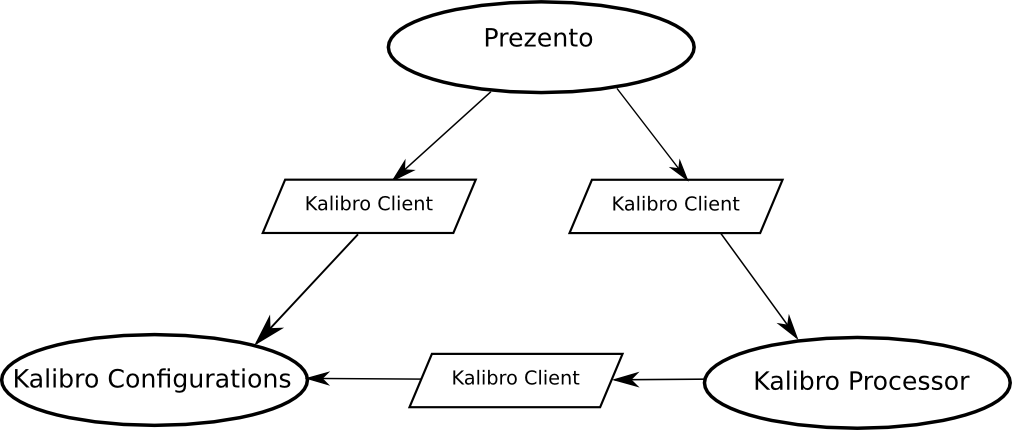
\includegraphics[scale=1.5]{figures/MezuroArchitecture.png}
                \label{fig:architecture}
            \end{center}
        \end{figure}
    \begin{itemize}
        \item Mezuro is composed of three parts:
            \begin{itemize}
                \item Configuration prior to the analysis
                \item Source code metrics computation and evaluation
                \item A graphic interface to present results
            \end{itemize}
        \item Currently, both the computation and visualization modules use
            other tools developed in the Mezuro project: \textbf{Kalibro} and
            \textbf{Prezento}

        \item Mezuro architecture evolved to a microservice architecture, to:
            \begin{itemize}
                \item Minimize maintainance cost
                \item Test and grant quality of code
                \item Require minimal previous knowledge from new contributors
            \end{itemize}
        \item \textbf{Kalibro} is the base of the architecture, and its
            segmented in three smaller entities:

            \begin{itemize}
                \item \textbf{Kalibro Processor}, responsible for processing and
                    evaluating metrics
                \item \textbf{Kalibro Configurations}, responsible for metrics
                    definitions and configurations
                \item \textbf{Kalibro Client}, responsible for all the communication
                    among the services
            \end{itemize}

        \item \textbf{Prezento}, the presentation layer, mainly communicates with
            Kalibro Processor and Kalibro Configurations, via the Kalibro
            Client interface
    \end{itemize}
\end{block}
